\documentclass[12pt]{article}
% packages that I call bc they are in the template I have and I don't know if I want them or not.
\widowpenalty=10000 
\clubpenalty=10000 
\usepackage{amsmath}
\usepackage{amsfonts}
\usepackage{amssymb}
\usepackage{wasysym}
\usepackage{graphicx}
\usepackage{pslatex}
\usepackage{lscape}
\usepackage{rotating}
\usepackage[T1]{fontenc}
\usepackage[latin1]{inputenc}
\usepackage{longtable}
\usepackage[font=scriptsize,labelfont=bf]{caption}
\setlength{\LTcapwidth}{5.5 in}
\usepackage{url}
\usepackage{lastpage}
\usepackage{lineno}
\usepackage[english]{babel}
\usepackage[usenames, dvipsnames]{color}
\usepackage[round, sort, numbers, authoryear]{natbib}
\usepackage{hyperref}
\usepackage{gensymb}
\usepackage{wrapfig}
\hypersetup{colorlinks,%
citecolor=black,%
filecolor=black,%
linkcolor=Mahogany,%
urlcolor=MidnightBlue,%
pdftex}

% header
\usepackage{fancyhdr}
\pagestyle{fancy}
 \rhead {\emph{\textcolor{blue}{bgetraer}, \thepage ~of
     \pageref{LastPage}}}
 \lhead{\footnotesize \textsc{GEO$/$Proposal for Junior Paper}}
 \cfoot{}
 \renewcommand{\headrulewidth}{0.4pt} 

% margins and linespacing
\textwidth = 6.5 in
\textheight = 8.84 in
\addtolength{\voffset}{-0.04in} 
\oddsidemargin = 0.0 in
\evensidemargin = 0.0 in
\topmargin =  0.0 in
\headheight = 0.1 in
\headwidth = 6.5 in
\headsep = 0.25 in
\parskip = 0.1 in
\parindent = 0.0 in
\linespread{1.25}

% define new commands for text that occur frequently
\newcommand{\MT}{^{\mathrm{MT}}}
\newcommand{\ga}{\gtrsim}
\newcommand{\Lpot}{(L+1)^2}
\newcommand{\WS}{^{\mathrm{WS}}}

% frontmatter 
\title{Spatial Localization of Greenland Mass Wasting Using a 2-D Wavelet Decomposition of GRACE Data and Comparison to Physical Drivers of Ice Loss}
\author{Benjamin Getraer}

\begin{document}
% Add line numbers
%\linenumbers

\maketitle

\begin{abstract}
Melting ice from the Greenland Ice-Sheet has accounted for an increasing percentage --- now estimated at over $25\%$ --- of rising global mean sea-level since the early 1990s. As recently as 2016, gravimetric and altimetric studies of Greenland melting rates found  increasing rates of ice loss, which have not been borne out in GRACE gravimetric observations over the last few years (2015--2017). We hypothesize that the true trend of Greenland ice loss between 2003--2017 is linear, and that deviations from the linear trend may be explained by inter-annual variability in climate. We demonstrate a novel application of 2-dimensional discrete wavelet analysis to the GRACE dataset to recover spatial structure of inter-annual variability in ice loss, focusing on the unusual melt and accumulation seasons of 2012--2014. Finally, we compare our interpretation of the 2012--2014 anomaly in spatial scale and location to the results of others using independent atmospheric, altimetric, and meteorologic data sources. \\[3em]

% see Mattingly for percentages
\textbf{Key Points:}
\begin{enumerate}
	\item We focus on inter-annual variability of the Greenland ice loss trend.
	\item We analyze the spatial structure of subregional signals in the GRACE dataset using discrete wavelet transforms.
	\item We define the 2012--2014 anomaly in spatial structure from the gravitational field.
\end{enumerate}

\textit{This proposal represents my own work in accordance with the Princeton University Honor Code. Note that this project is a continuation of work from my Spring 2018 Junior Paper and some text and figures appear in this proposal from that paper.\\
My adviser is Laure Resplandy and I plan on having Frederik Simons as a second reader when he is available again in the Spring.}

\end{abstract}

\section{Introduction \label{sec:introduction}}

Average global surface temperature is rising at an increasing rate --- approximately $0.09\degree$~C per decade since 1880, and approximately $0.26\degree$~C per decade since 1979 \cite[][]{ipcc2013_atmosphere}
--- and has contributed to significant melting of the
Greenland ice sheet, with recent ice loss approximated at $-244$~Gt per
year \cite[][]{Harig+2015a,Harig+2016}. The Greenland Ice Sheet covers just over 1\% of
Earth's surface, and, if completely melted, would raise sea level by over $7$~m
\cite[][]{ipcc2013_cryosphere}.
Massive loss of ice has
significant repercussions for human civilization, bringing with it a rising sea
level at about $1$--$2$~mm per year at the end of 2010
\cite[][]{ipcc2013_sealevel}.  Our broad goal is to understand deviations from modeled rates of Greenland ice melt in order to better understand, predict, and
communicate the changing conditions of the planet.


\begin{figure}[h!]
\centering
\makebox[\textwidth][c]{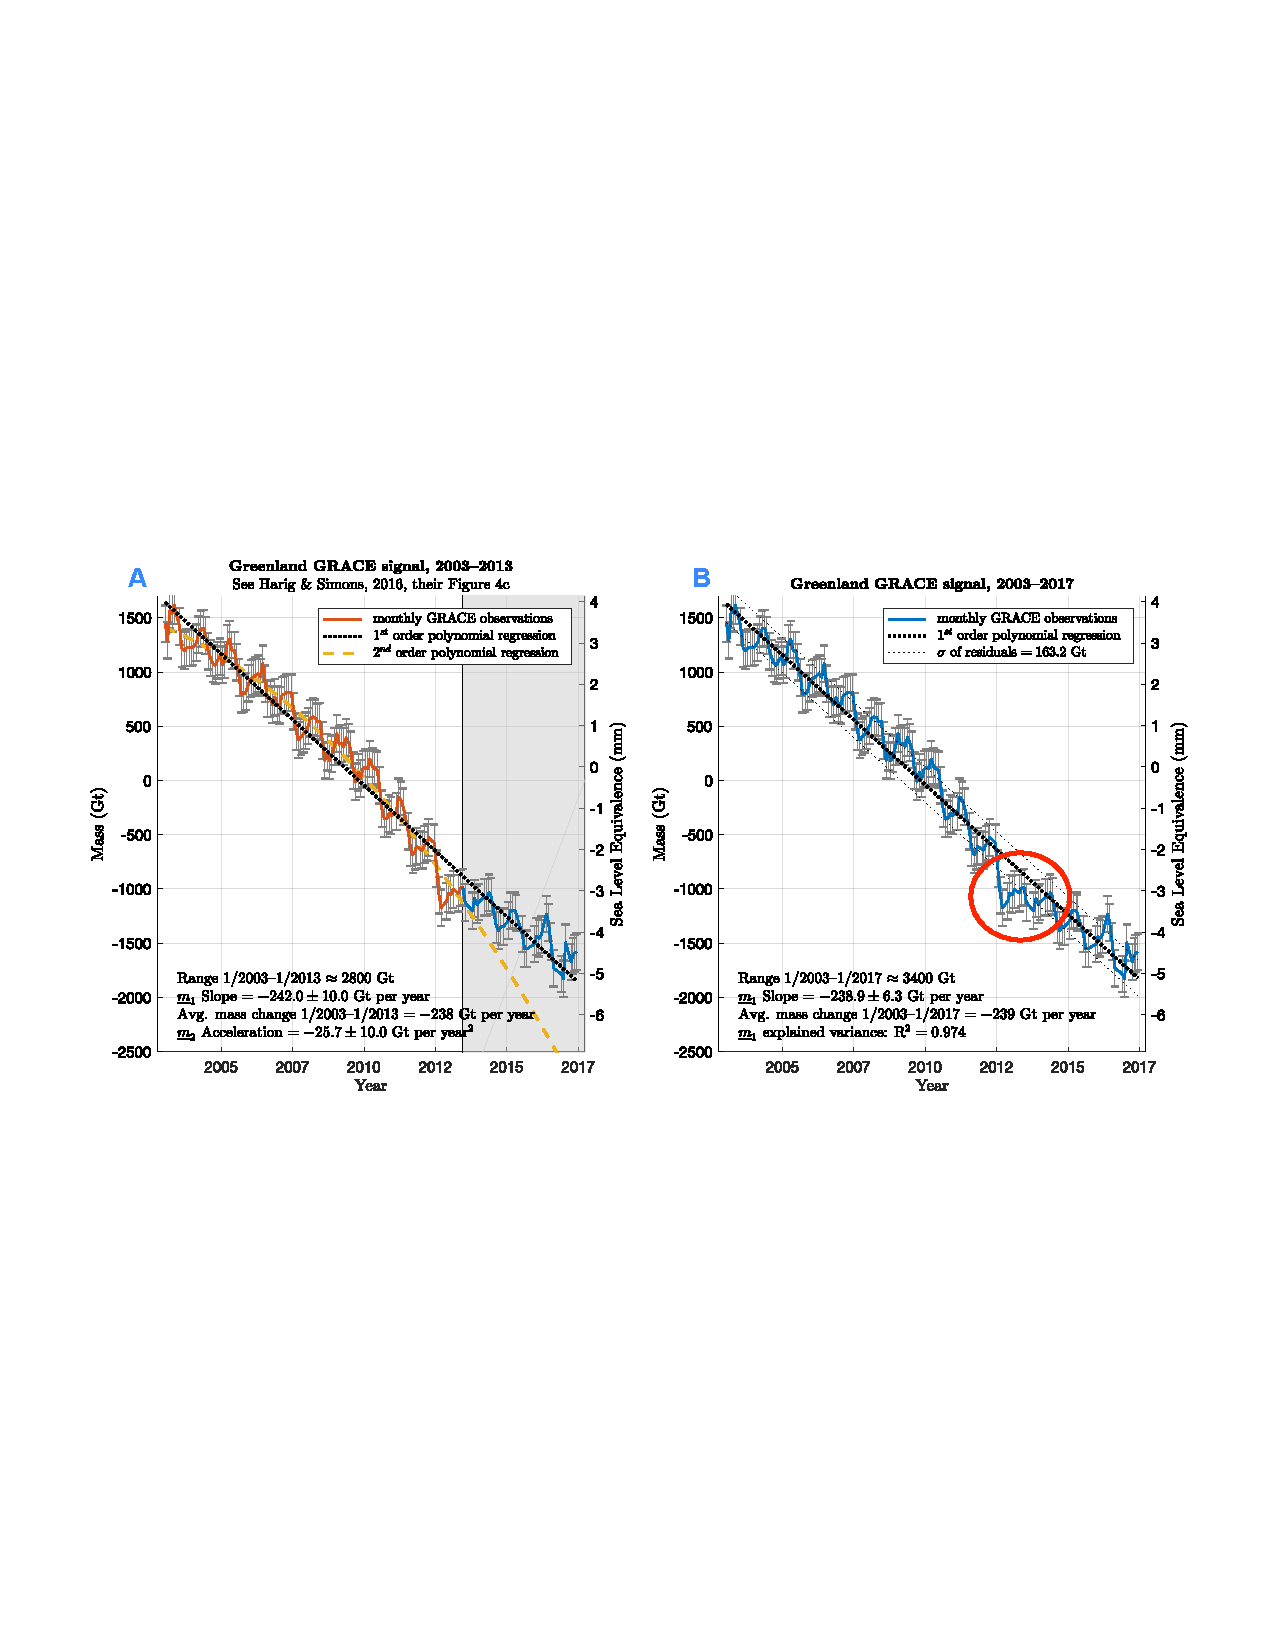
\includegraphics[height=0.37\textheight]
{Figures/HarigGetraerTrend.pdf}}
\caption[Greenland Mass Trend: 2003--2017]{Total mass changes for Greenland over the complete GRACE record using equivalent methods to \cite{Harig+2016}. Shown in \textbf{A} are the $\underline{m}_1$ (linear) and $\underline{m}_2$ (quadratic) models for 01/2003--06/2013, comparable to previous estimates of the mass trend \citep{Harig+2016}. Note the significant departure of the extrapolated $\underline{m}_2$ model from the continuing signal. Shown in \textbf{B} is the $\underline{m}_1$ linear model for 01/2003--06/2017 with the standard of deviation of its residuals. Note that the $\underline{m}_1$ model does not significantly change after including the entire GRACE record. Error bars represent $2\sigma$ based on the combined variance of modeled Slepian coefficients $f_{\alpha}$ (see \cite{Harig+2016}, as well as my Fall and Spring JPs). This Figure appeared in my Fall and Spring JP, here with minor updates.} \label{fig:Getraer}
\end{figure}

Ice mass on the Greenland Ice Sheet has been calculated using
gravimetric data from NASA's Gravity
Recovery and Climate Experiment (GRACE), as well as satellite and airplane based
altimetry, finding decreasing rates in the ice mass signal over the last
decade \cite[][]{khan2015,Harig+2016}. Rates of ice loss increase by a
combination of greater discharge from calving glacier termini at the edges of
the ice-sheet and decreased surface mass-balance, the difference between
seasonal snow accumulation and melting \cite[][]{khan2015,enderlin2014}.
Significant inter-annual variability and asynchronicity has been observed in
the discharge rates of the Greenland Ice Sheet's major drainage basins, while
surface mass-balance is comparatively more predictable
\cite[][]{mcmillan2016,enderlin2014}. Both contributions to ice loss accelerated between 2000--2012, combining for a total acceleration of ice mass
estimated around $-30$~Gt per year$^2$ over all of Greenland
\cite[][]{velicogna2009,enderlin2014}.

\begin{wrapfigure}{r}{0.5\textwidth} 
%\vspace{-50pt}
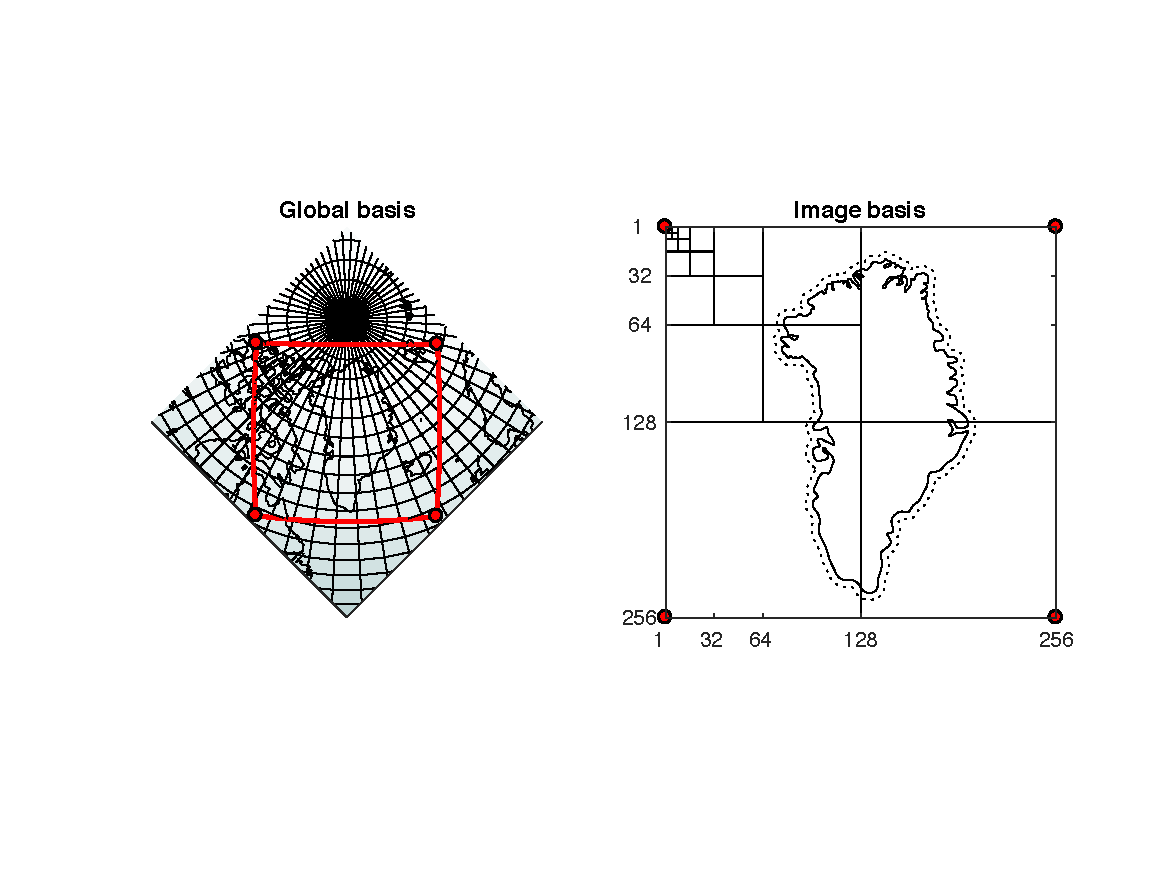
\includegraphics[width=1.1\linewidth]{Figures/thegrid.pdf}
\caption[The Discrete Grid Around Greenland]{A grid around Greenland is defined in the global basis on a face of the Cubed Sphere centered on Greenland on which the GRACE spherical harmonic data are solved. In the image basis the grid is cartesian with length $256$. Grid lines in the image basis represent the diminishing spatial support of wavelets of different levels, from $\zeta=8$ (the entire image) to $\zeta=1$ (a unit grid cell). Note that in reality, each wavelet level has coverage over the entire image. The dotted line around Greenland is a coastal buffer of $0.5^{\circ}$ as in \cite{Harig+2016}. This Figure appeared in my Spring JP.} \label{fig:thegrid}
%\vspace{-50pt}
\end{wrapfigure}

A study by \cite{Harig+2016} modeling the mass of the Greenland Ice Sheet
using GRACE data products showed deviations from the long-term quadratic
trend, starting with a high level of melt in the summer of 2012, and followed by two
summers of little melting in 2013 and 2014 \cite[see
Figure~\ref{fig:Getraer} A, comparable to][their
Figure~4]{Harig+2016}. Our analysis of the complete GRACE data set (2002--2017) using the same methods showed a linear,
 not accelerating, trend of ice loss for the Greenland Ice Sheet, constraining the observed unexpected deviations to an unusually large melt summer of 2012 followed by a summer of unusually little melt in 2013 (see
Figure~\ref{fig:Getraer} B). 



The anomalous seasons of 2012--2013 have received attention in recent literature by studies attempting to understand how surface mass balance processes could produce such inter-annual variability. Explanations and correlations have been found relationships with climate indices such as the phase of the North Atlantic Oscillation \cite[][as well as my Fall 2017 JP]{mcmillan2016,bevis2018}, transient atmospheric transport of water vapor in so-called "atmospheric rivers" \citep{mattingly2018}, and non-radiative energy flux caused by short-term cloud cover \citep{solomon2017}. 

\subsection{Previous Results \label{sec:prevresults}}
In my Spring 2018 JP, I explored the use of a 2-D wavelet basis to represent the GRACE gravimetric data over Greenland such that meaningfully contributing basis functions also contained information about spatial structure (see
Figure~\ref{fig:thegrid}). 

I developed a procedure for choosing the most important wavelet basis functions in order to extract the true fluctuation of the signal from the over-determined image calculated from the typical GRACE spherical harmonic basis. I then tested which wavelet basis function best captured the 2012--2013 deviation from the expected signal, finding the deviations to be concentrated in southwestern Greenland (see
Figure~\ref{fig:deviant}). 



\begin{wrapfigure}{r}{0.5\textwidth} 
%\centering
%\makebox[\textwidth][c]{
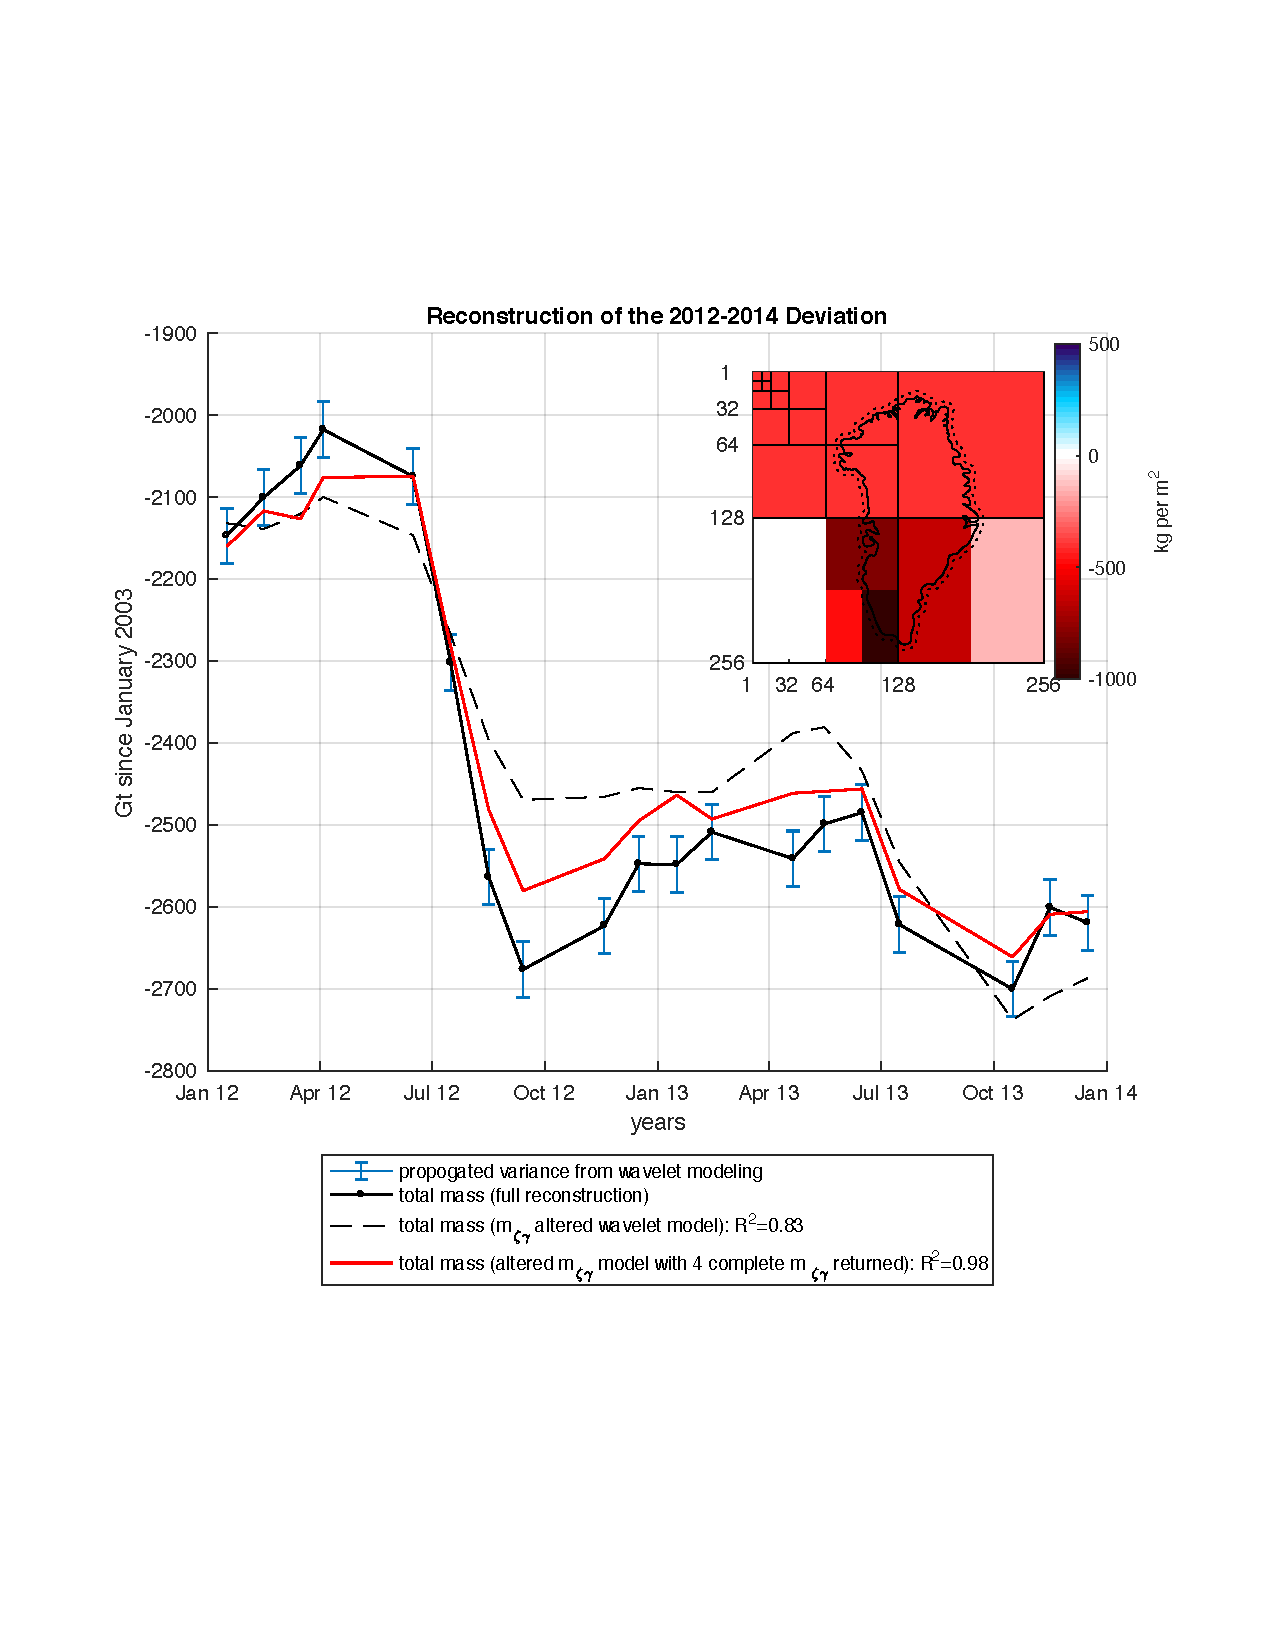
\includegraphics[width=\linewidth]{Figures/deviant.pdf}
%}
\caption[Location of the 2012--2014 Deviation]{The 2012--2014 deviation in Greenland mass and the total from the reconstructed modeled wavelet coefficients. By adding in the real values of only four wavelet coefficients back into the modeled wavelet reconstruction we improve the variance explanation by $15\%$. These wavelets are shown inset, weighted by their values in September 2012, the extreme of the deviation, and are concentrated in southwestern Greenland. ``m$_{\zeta\gamma}$'' refers to a wavelet basis function ``m'' of index $\gamma$ in level $\zeta$. This Figure appeared in my Spring JP.
\label{fig:deviant}}
\end{wrapfigure}

\section{Objectives and Methods \label{sec:methods}}
This paper aims for two objectives. First, to justify and demonstrate a different way of examining the gravitational signal represented in the GRACE dataset published by NASA; Second, to apply this new method to the signal of Greenland mass wasting to test the results of this method when pushed to resolve spatial and temporal variation of the signal within the spatial footprint of Greenland. 

Both of these objectives have been worked towards in my previous work, and my overarching goal in this thesis is to situate my work more clearly in the context of and in conversation with the results of others working on similar problems. I will continue to refine and experiment with my methods relating to basis functions and representation in the wavelet domain, while testing my results against the findings of others. As mentioned, many recent papers have discussed the 2012--2013 melt seasons of the Greenland Ice Sheet, and I plan on mining through their figures and supplementary data to compare to my spatial and temporal results for those anomalies (for example:  \cite{mattingly2018,solomon2017,mcmillan2016,bevis2018,fausto2016, hanna2014}. Between my continued refinement and justification of method and thorough contextualization with the current best understanding of Greenland Ice Sheet melt events, the value of this rather novel application of 2-dimensional wavelets to the GRACE dataset can be properly determined.

\section{Budget Justification \label{sec:budget}}

All data, code, sources, and software that will be used are either
publicly available for free or already made available under licensing
from Princeton University at no additional expense. The entirety of
this project will be in data analysis and computer modeling, and no
travel, data, or consumable supplies costs are anticipated.
 
\section{Acknowledgements \label{sec:ack}}

Thank you to my Senior Thesis adviser Professor Laure Resplandy for taking on this project with me. Thank you to my Junior Paper adviser Professor Frederik J.~Simons whose patience and passion gave me the tools and confidence to pursue my interests and contributed greatly in the conceptualization and direction of this project. Thank you to the second reader of my Fall Junior Paper, Prof.~Jessica Irving for feedback, suggestions, and encouragement. Thanks to Dr.~Amanda
Irwin Wilkins and ``The Hare'' writing workshop group for discussing
and editing various figures and drafts. Thank you to Prof.~Adam C.~Maloof who taught me \LaTeX, and to Dr.~Chris Harig for providing some of the data files. Thank you to Prof.~Gabriel Vecchi for insight into atmospheric and oceanic processes. Thank you to Jean Getraer, Andrew Getraer, Jonathan Feld, Rae Perez, and Zach Smart for proof-reading various drafts of my Junior year work.  Lastly, thank you to the numerous professors and graduate students in the Princeton Department of Geosciences and at Princeton Research Day for feedback, encouragement, and constructive criticism on the presentation of preliminary results.

% References
\small
\renewcommand{\bibsep}{0em}
\renewcommand{\bibname}{References}
\bibliographystyle{/Users/benjamingetraer/Documents/SeniorThesis/senior-thesis/LatexFiles/gji}
\bibliography{/Users/benjamingetraer/Documents/SeniorThesis/senior-thesis/LatexFiles/bgetraerThesis}

\end{document}
